
\documentclass[fleqn,12pt]{article}

\usepackage[margin=15mm]{geometry}
\usepackage[utf8]{inputenc}
\usepackage[bulgarian]{babel}
\usepackage[unicode]{hyperref}
\usepackage{amsfonts}
\usepackage{amssymb}
\usepackage{enumitem, hyperref}
\usepackage{upgreek}
\usepackage{indentfirst}
\usepackage{graphicx}

\usepackage{amsmath}

\graphicspath{ {./img/} }

\title{Тема 15\\ Модели на разпределени софтуерни архитектури. Среди и протоколи за разпределени приложения.}

\author{v0.1}
\date{25 юни 2021}

\begin{document}

\maketitle
\tableofcontents
\pagebreak

\section{Параметри на паралелната и разпределената обработка}

\subsection{Дадености}

\textbf{\textit{Разпределените (Дистрибутираните) системи}} са системи съставени от множество процеси разположени върху различни мрежови възли.
За краткост ще казваме възел когато имаме предвид мрежови възел.
Съставните компоненти комуникират помежду си чрез изпращане на съобщения посредством \textbf{IPC} методи.
\bigbreak
\textbf{\textit{Споделена памет}} между процеси наричаме памет, която е заделена върху точно един възел и може да бъде достъпена само от процесите върху него посредством шината на дънната платка.
\bigbreak
\textbf{\textit{Разпределена (Дистрибутирана) памет}} между процеси наричаме памет, която е задалена върху няколко възела и може да бъде достъпена чрез обмен на съобщения.
\bigbreak
\textbf{\textit{Паралелна обработка}} (\textit{Parallel computing}) наричаме обработка, при която една задача се разделя на подзадачи, които се изпълняват едновременно от няколко процесора.
Паметта между процесите при паралелната обработка може да е както споделена така и разпределена.
Задачите при паралелната обработка са tightly-coupled.
Чрез нея се спестява време.
\bigbreak
\textbf{\textit{Разпределена (Дистрибутирана) обработка}} (\textit{Distributed computing}) наричаме обработка, при която една задача се разделя на подзадачи, които се изпълняват върху различни възли.
Паметта между процесите при разпределена обработка може да е само разпределена.
Задачите при разпределената обработка са loosely-coupled.
Чрез разпределена обработка се постига стабилност.
\bigbreak
\textbf{\textit{Заб.}} - Една разпределена система може да включва както паралелна, така и разпределена обработка.

\subsection{Паралелни алгоритми и закон на Амдал}

\textbf{\textit{Сериен алгоритъм}} е алгоритъм, който може да изпълнява максимум една операция в даден момент.
Сложността може да се изчислява като функция на размера на входа.
\bigbreak

\textbf{\textit{Паралелен алгоритъм}} е алгоритъм, който може да изпълнява няколко операции едновременно.
Сложността може да се представи като функция на архитектурата и средата за паралелна обработка.

\bigbreak
Основните характерстики на паралелните алгоритми, които ги отличават от серийните са:
\begin{itemize}
    \item Брой процеси и логическата им организация
    \item Разпределение на данните и модел на техния обмен
    \item Точки на синхронизация на процесите
\end{itemize}
\bigbreak

За всеки алгоритъм е изпълнено, че не всяка негова част може да бъде паралелизирана.
Следователно не можем да ускоряваме до безкрайност.
\textbf{Законът на Амдал} гласи, че 
\begin{center}$S_{latency}(s) = \frac{1}{(1-p) + \frac{p}{s}}$, \end{center}
където:
\begin{itemize}
    \item $S_{latency}$ е теоретичното ускорение на изпълнението на цялата задача.
    \item $s$ е ускорението на секцията, която паралелизираме.
    \item $p$ е фракцията от времето на задачата заемано от секцията, която сме паралелизирали, при серийно изпълнение на алгоритъма.
\end{itemize}

\subsection{Метрики и методи за анализ на паралелните алгоритми}

\textbf{\textit{Степен на паралелизъм $p$}} в даден момент е максималният брой операции, които могат да се изпълняват паралелно при обработката на алгоритъма.
Т.е. процеси/нишки респективно брой ядра/възли.
\bigbreak
\textbf{\textit{Ускорение (acceleration)}} пресмятаме чрез $S_p = \frac{T_1}{T_p}$, където $T_1$ е времето за серийна обработка, а $T_p$ е времето за паралелна обработка при степен на паралелизъм $p$.
Поради наличие на комуникационни и синхронизационни закъснения $S_p \in (1, p)$.
\bigbreak
\textbf{\textit{Ефективност (efficiency)}} е частта от общото време за паралелна обработка, през която процесорите се използват ефективно.
Изразява се чрез $E_p = \frac{S_p}{p} = \frac{T_1}{pT_p}$, като $E_p \in (0, 1)$, където $S_p$ е ускорението, а $p$ е степента на паралелизъм.
\bigbreak
\textbf{\textit{Цена (cost)}} е времето отнето от процесорите за изпълнение на алгоритъма. Измерва се, чрез $C_p = pT_p$, където $T_p$ е времето за паралелна обработка при степен на паралелизъм $p$.
\bigbreak

\textbf{\textit{Грануларност}} е количеството работа за извършване на подзадачите, на които се разбива задачата на алгоритъм при паралелна обработка.
Тя може да се измерва във време използвайки следната формула $G = \frac{T_{comp}}{T_{comm}}$, където $T_{comp}$ е времето прекарано в изпълнение на подзадачите, а $T_{comm}$ е времето прекарано в комуникация между процесите.
Има няколко вида грануларност:
\begin{itemize}
    \item \textit{Фина}, където задачата се разбива на огромен брой малки подзадачи, които могат да се извършват паралелно.
    По този начин работата се разпределя равномерно между процесорите, което резултира в баланс на натоварването (\textit{load balancing}).
    Препоръчително е да се изолзва при $``$дисбалансирани$''$ данни за обработка, както и при наличие на бърза комуникация с малко \textit{overhead}, като при \textit{shared memory}.
    \item \textit{Едра}, където задачата се разбива на малък на брой големи подзадачи, които могат да се извършват паралелно.
    По този начин може да се стигне до дисбаланс между работата на процесорите.
    Препоръчителное да се използва при $``$балансирани$''$ данни за обработка, както и при наличие на бавна комуникация с много \textit{overhead}, като при \textit{message pasing}.
    \item \textit{Средна}, която е компромис между фината и едрата грануларност.
    Тя е най-често срещаната.
\end{itemize}
\bigbreak

Паралелните алгоритми се делят на асинхронни, локално синхронни и глобално синхронни.
\bigbreak

При разпределените системи топологията на разпределение на процесите влияе върху балансирането на натоварването между възлите. Тя може да бъде:
\begin{itemize}
    \item \textit{централизирана} - напр. звезда.
    \item \textit{йерархична} - напр. дървета
    \item \textit{разпределена} - напр. верига, решетка и хиперкуб.
\end{itemize}

\subsubsection{Аномалии при паралелните алгоритми}

\textbf{\textit{Суперлинейна аномалия}} наричаме случая когато $S_p > p$.
Тя може да се наблюдава при наличие на неоптимален сериен алгоритъм или при нисък капацитет на хардуер.
Пример е когато при серийна обработка данните заемат твърде много оперативна памет и се наложи използването на swap памет, докато при паралелна обработка данните заемат много по-малко памет и изчисленията се извършват изцяло с оперативната памет.

\textbf{\textit{Немонотонна аномалия}} наричаме случая когато $\exists p: S_p > S_{p+1}$.

\section{Модели на разпределените софтуерни архитектури и техните структури, организация, компоненти и приложение}


\textbf{\textit{Софтуерната архитектура}} дефинира какви са съставните процеси на една софтуерна сисмета, как те са структурирани и си взаимодействат.
\textbf{\textit{Моделите на софтуерни архитектури}} представляват богати на информация и точни диаграми, описващи дизайна на системата.
Под дизайн се разбира съвкупността от декомпозицията на съставните компоненти, техните функции, прилагания архитектурен стил и качествени атрибути.

\subsection{Процедурни модели}

\textbf{\textit{Процедурните архитектурни модели}} се базират на разпределена обработка чрез \textit{отдалечено извикване на процедури (remote procedure call (\textbf{RPC}))} или \textit{Remote Method Invocation (\textbf{RMI})}.
Представлява извикване на процедура на един възел от друг възел, като това това е прозрачно за извикващия възел, т.е. е като локална за него процедура.

\subsection{Обектни модели}

\textbf{\textit{Обектно-ориентираните архитектурни модели}} се основават на разделянето на отговорностите на системата в индивидуални повторно използваеми и независими обекти, които си сътрудничат.
Основните принципи на тези модели са:
\begin{itemize}
    \item \textit{Абстракция} - опростяването на решението на реален проблем чрез дефиниране на подходящи класове.
    \item \textit{Композиция} - изграждането на обекти от други обекти.
    \item \textit{Наследственост} - автоматичното присвояване на функционалностите на едни обекти на други обекти и тяхното разширение и промяна.
    \item \textit{Капсулация} - скриването на ненужните за потребителя детайли на някои обекти.
    \item \textit{Полиморфизъм} - присвояването на едно и също име на различни операции на клас или йерархия от класове.
\end{itemize}

\subsection{Потокови модели}

\textbf{\textit{Потоковите архитектурни модели}} разглеждат системата като последователност от трансформации на последователен набор от данни.
Всеки компонент трансформира входните си данни в изходни.
Топологията на пренос на данните между тях се задава експлиситно чрез \textbf{блок-диаграми}.
Модулите поддържат само интерфейс по данни, но не и контролен, като те не се адресират директно, а чрез предаваните данни.
\bigbreak
По механизма на свързване между модулите се разграничават:
\begin{itemize}
    \item \textit{Пакетна обработка (Batch Sequential)} - Модулите се извикват в последователен ред един след друг, като изходът от един модул се предава като вход на следващия.
    Пакетите от данните които обработват от всеки модул са записани под формата на временни файлове, които служат за комуникация между два последователни в изпълнението си модули. 
    Най-често този модел се използва за асинхронна обработка на данни, като се цели оптимално използване на ресурси за сметка на паралелизъм и интерактивност.
    \begin{center} 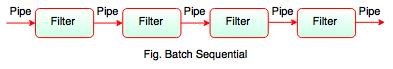
\includegraphics[width=300px]{batch_sequential.jpg} \end{center}
    \item \textit{Филтрирани канали (Pipe and Filter)} - модулите се делят на филтри, канали, източник на данни и консуматор на данни.
    Каналите са потоци от данни изпълняващи ролята на конектори между филтрите. 
    Филтрите са модули, трансформиращи входните си данни, които могат да работят паралелно и независимо едни от други, като всеки филтър започва предава изходните данни към следващия филтър преди да е свършил с обработката на всичките данни.
    Този начин за обработка на данни позволява паралелизъм (конвейеризация).
    \begin{center} 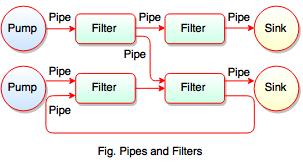
\includegraphics[width=220px]{pipe_and_filter.jpg} \end{center}
    \item \textit{Контролни процеси (Process Control)} - декомпозира системата на модули като потока на данните идва от множество променливи, което управлява реда на изпълнение на процеса.
    \textit{Контролните процеси} позволяват обработка чрез паралелизъм (конвейеризация) и са подходящи за системи в реално време.
\end{itemize}

\subsection{Контекстни (Data centric) модели}

\textbf{\textit{Контекстните архитектурни модели}} се характеризират с централизирано хранилище за данните, от където те са достъпни за всички останали компоненти на системата.
Декомпозицията на модулите се състои от модул за \textbf{управление на достъпа до данните} и \textbf{агенти}, които извършват операции върху тях.
\bigbreak
Интерфейсът между агентите и данните може да бъде явен (при \textbf{RMI} и \textbf{RPC}) или имплицитен (напр. \textbf{транзактивен}).
В оригинал не се предвижда комуникация между агентите.
\bigbreak
Съществуват два основни контекстни модела:
\begin{itemize}
    \item \textit{Хранилище (Repository)}, където агентите са активни. Примери са СУБД, CORBA и UDDI.
    \item \textit{Черна дъска (Blackboard)}, където инициативата е на модула с данните, а агентите се абонати за събития (\textit{event listeners}).
    Събитие настъпва при промяна в данните.
    Използват се при AI-разпределени системи и ERP като складови и транспортни системи.
\end{itemize}

\subsection{Йерархични модели}

\textbf{\textit{Йерархичните архитектурни модели}} декомпозират системата на йерархични модули, като функциите се групират по йерархичен принцип на няколко нива.
Координацията обикновено е между модули от различни нива (вертикална свързаност) и се базира на явни (т.е. "заявка-отговор") обръщения.
Слоевете делегират своята работа на услуги от съседни по-ниски нива.
Пълна прозрачност между нивата се постига при запазване на свързващите интерфейси.
\bigbreak
Начини за имплементация са:
\begin{itemize}
    \item \textit{Слоест модел} - използван при много ОС като Unix, GNU и Windows.
    Също така протоколните стекове OSI и TCP/IP са слоести архитектури.
    \item \textit{Йерархия с подпрограми (Main/Subroutine)} - разделя комплексни задачи на по-малки задачи, които се изпълняват от подпрограми.
    Главната програма оркестрира обръщенията към подпрограмите.
    Пример за такъв модел е \textbf{Master/Slaves} архитектурата.
\end{itemize}

\subsubsection{Master/Slaves}

\textbf{\textit{Master/Slaves}} е йерархия с подпрограми, поддържаща следните качества:
\begin{itemize}
    \item отказоустойчивост и надеждност
    \item балансиране на натоварването между робите за по-ускорено изпълнение
\end{itemize}

Състои се от един господар \textbf{M}, който разбива задачата на подзадачи и заповядва на робите $S_1, \dots, S_n, n \in \mathbb{N}$ да ги изпълняват.
Ролята на \textbf{M} е да:
\begin{itemize}
    \item оцени годността на паралелно обработените резултати от $S_n$, използвайки протоколи за отказоустойчивост, идентифициращи грешните и верни резултати.
    \item балансира натоварването между робите.
\end{itemize}

\begin{center} 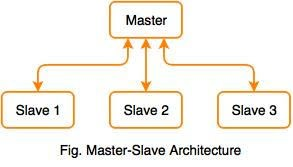
\includegraphics[width=220px]{master_slave.jpg} \end{center}

\subsection{Асинхронни модели}

\textbf{\textit{Асинхронните модели}} се базират на имплиситни асинхронни обръщения между обслужващите процеси.
\bigbreak
Асинхронният обмен може да бъде от тип \textbf{Producer/Consumer}, където обменът на данни е 1:1.
Има следните разновидности:
\begin{itemize}
    \item \textit{интерактивeн (online)}, където няма буфериране и и двата процеса са активни
    \item \textit{отложен (offline)}, където обмена на съобщенията се опростява посредством процес-буфер.
    Това позволява консуматора да не е активен по време на изпращане на съобщения, както и обратното.
\end{itemize}
\bigbreak
\textbf{Publisher/Subscriber} също е вид асинхронен обмен на съобщения където обменът на данни е 1:*.
Има следните разновидности:
\begin{itemize}
    \item \textit{topic-based}, където съобщенията се изпращат до topic-и, които са именувани канали.
    Издателят е отговорен за дефинирането на topic-ите, а абонатите получават съобщенията от всички topic-и, за които са се абонирали.
    \item \textit{content-based}, където съобщенията се изпращат до абонат, ако атрибутите на съдържанието отговарят на ограниченията дефинирани от абоната.
    Абонатът е отговорен за класификацията на съобщенията.
\end{itemize}

\subsection{Интерактивни модели}

\textbf{\textit{Интерактивните модели}} поддържат интензивен потребителски интерфейс.
За целта декомпозицията на системата е на 3 функционални модула:
\begin{itemize}
    \item \textit{модул за представяне (изглед)}, имплементиращ потребителския интерфейс.
    Използва се за представяне (в т.ч. графично и мултимедийно) на изходните данни и намеса на потребителите в обработката (т.е. вход за данни и контрол)
    \item \textit{модул данни}, поддържащ данновия модел заедно с базова функционалност за обработката на данните
    \item \textit{модул за управление}, който отговаря за системни комуникации, управление на процесите, инициализиране и конфигуриране на модули данни, както и управление на изгледи.
\end{itemize}

Има две категории интерактивни софтуери архитектури - \textbf{PAC (Presentation-Abstraction-Control)} и \textbf{MVC (Model-View-Controller)}, където аналогията между \textbf{P-V, A-M, C-C}.
Те се различават по начина на управление като:
\begin{itemize}
    \item \textbf{PAC} е с йерархично (разслоено) и разпределено управление, при което системата се формира от набор коопериращи агенти на три нива - \textbf{базово ниво}, състоящо от агенти работещи върху общи данни и бизнес логика, \textbf{средно ниво}, състоящо от агенти координатори на изгледите и \textbf{ниво на изгледите} за обработка на локални данни.
    Всеки агент имплементира \textbf{P, A и C} компоненти.
    \begin{center} 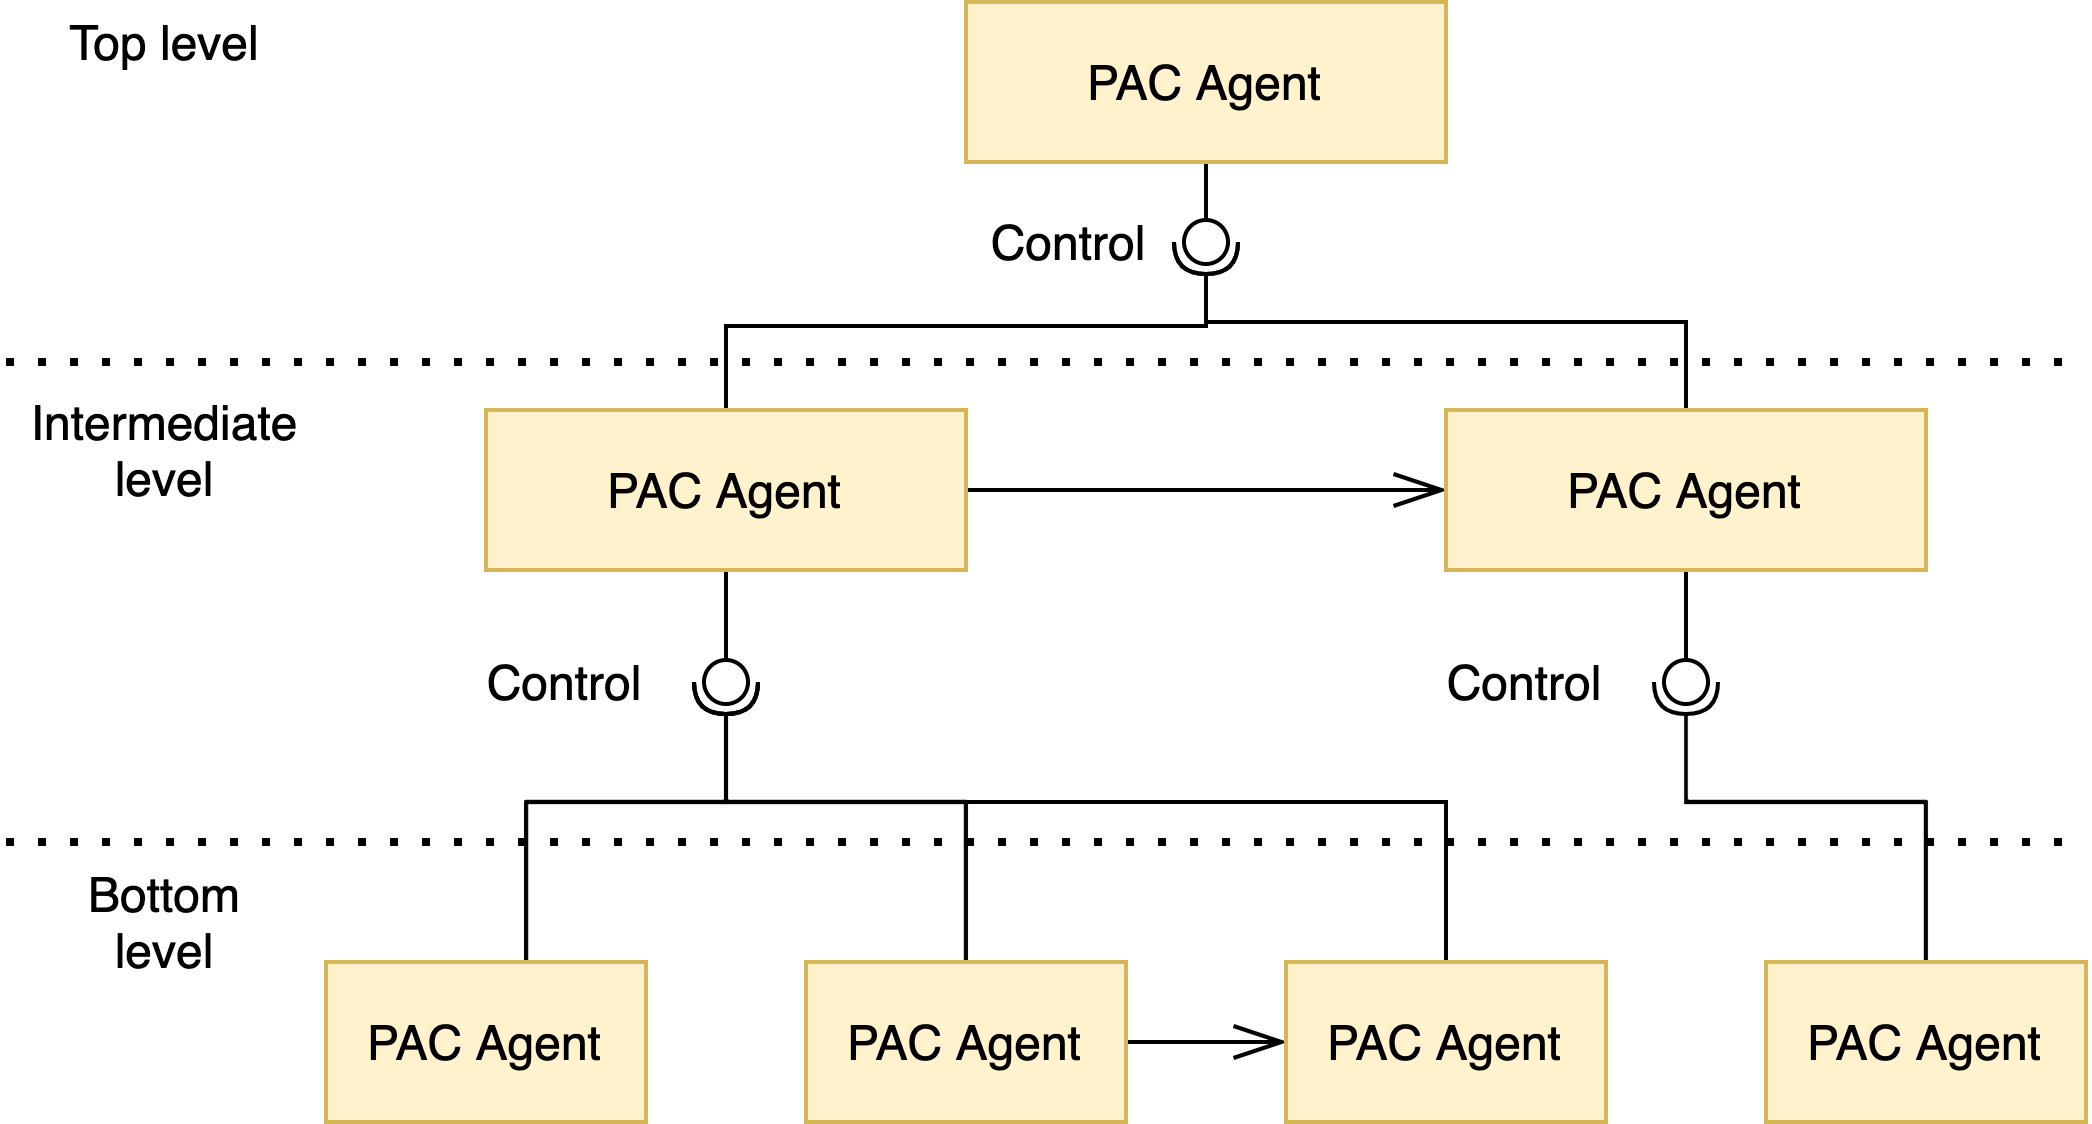
\includegraphics[width=250px]{pac.png} \end{center}
    \item при \textbf{MVC} агентите са равнопоставени.
\end{itemize}

\section{Организация на разпределените приложения}

\textbf{\textit{Multiple programs multiple data (MPMD)}} наричаме разпределени системи състоящи се от много програми паралелно извършващи работа върху различни данни.
Използват се при наличие на множество потребители, като системи за масово обслужване.

\subsection{Клиент-сървър и двуслойни архитектури}

\textbf{\textit{Клиент-сървър}} е класически \textbf{MPMD} модел за адаптиране на ограничена клиентска инфраструктура към сложни задачи.
Процесите се класифицират като два основни:
\begin{itemize}
    \item \textit{Сървър}, който е реактивен процес, имплементиращ приложната логика и данновия модел под формата на конкретен набор от услуги.
    \item \textit{Клиент}, който е активен интерфейсен процес, използващ услугите на сървъра.
\end{itemize}

Има два основни вида клиенти - \textbf{тънки (thin)}, които делегират цялата работа на сървъра, и \textbf{дебели (fat)}, които изпълняват част от задачата.
\bigbreak


\begin{center}
\begin{tabular}{ |c|c| } 
    \hline
    Предимства & Недостатъци \\
    \hline
    технологично специализиране & унификация на клиентската инфраструктура \\
    \hline
    инфраструктурна гъвкавост (скалиране) & по-трудна защита на достъпа до данние \\
    \hline
    преизползване & скалируемост на сървъра \\
    \hline
    еволюция без участието на потребителя & скъпа поддръжка, профилактика и тестване \\
    \hline
\end{tabular}
\end{center}

\subsection{N-слойни архитектури}

\textbf{\textit{N-слойната архитектура}} включва надграждане над клиент-сървър архитектурата, където компонентите са разделени на няколко слоя.
Можем да си представим, че слоевете са вертикално подредени и компонентите на даден слой са клиенти на сървъри от съседния долен слой.
\bigbreak
При \textbf{N-слойните архитектури} редовно се срещат \textbf{многослойни сървъри}, където сървърната част е декомпозирана на поне два слоя, които се класифицират като:
\begin{itemize}
    \item \textit{междинни слоеве}, които се намират между интерфейсния и вътрешния слой, имплементиращ $``$бизнес логиката$''$.
    \item \textit{вътрешен слой}, най-долният слой, който обичайно е персистентен или се използва за комуникации. 
\end{itemize}

Очевидно щом е надграждане над клиент-сървър архитектурата, то \textbf{\textit{N-слойната}} разполага със същите недостатъци и предимства, но по-силно изразени.
\bigbreak
\textbf{\textit{3-слойните архитектури}} са вид \textbf{N-слойни}, където имаме наличието на интерфейсен, междинен и вътрешен слой.

\subsection{Peer-to-Peer архитектури}

\textbf{\textit{Peer-to-Peer (P2P) архитектурата}} се разгръща като \textbf{наслоена (overlay) мрежа} върху съществуваща клиентска част от мрежова инфраструктура.
Всеки участник е еднакво прелигирован и заделя част от ресурсите си (cpu, диск и др.), който да се използва от останалите участници в мрежата без нуждата от каквато и да е централна координция.
За разлика от класическата архитектура клиент-сървър всеки участник изпълняват фукцията на клиент и сървър едновременно за другите участници.
\textbf{P2P} се характеризира чрез \textbf{децентрализирана топология}, \textbf{самоорганизация}, \textbf{инцидентна (ad hoc) и динамична свързаност и наличност} на възлите и процесите в тях, \textbf{скалируемост}, \textbf{отказоустойчивост (fault tolerance)}, анонимност на споделянето и специална юридическа регулация.

\begin{center} 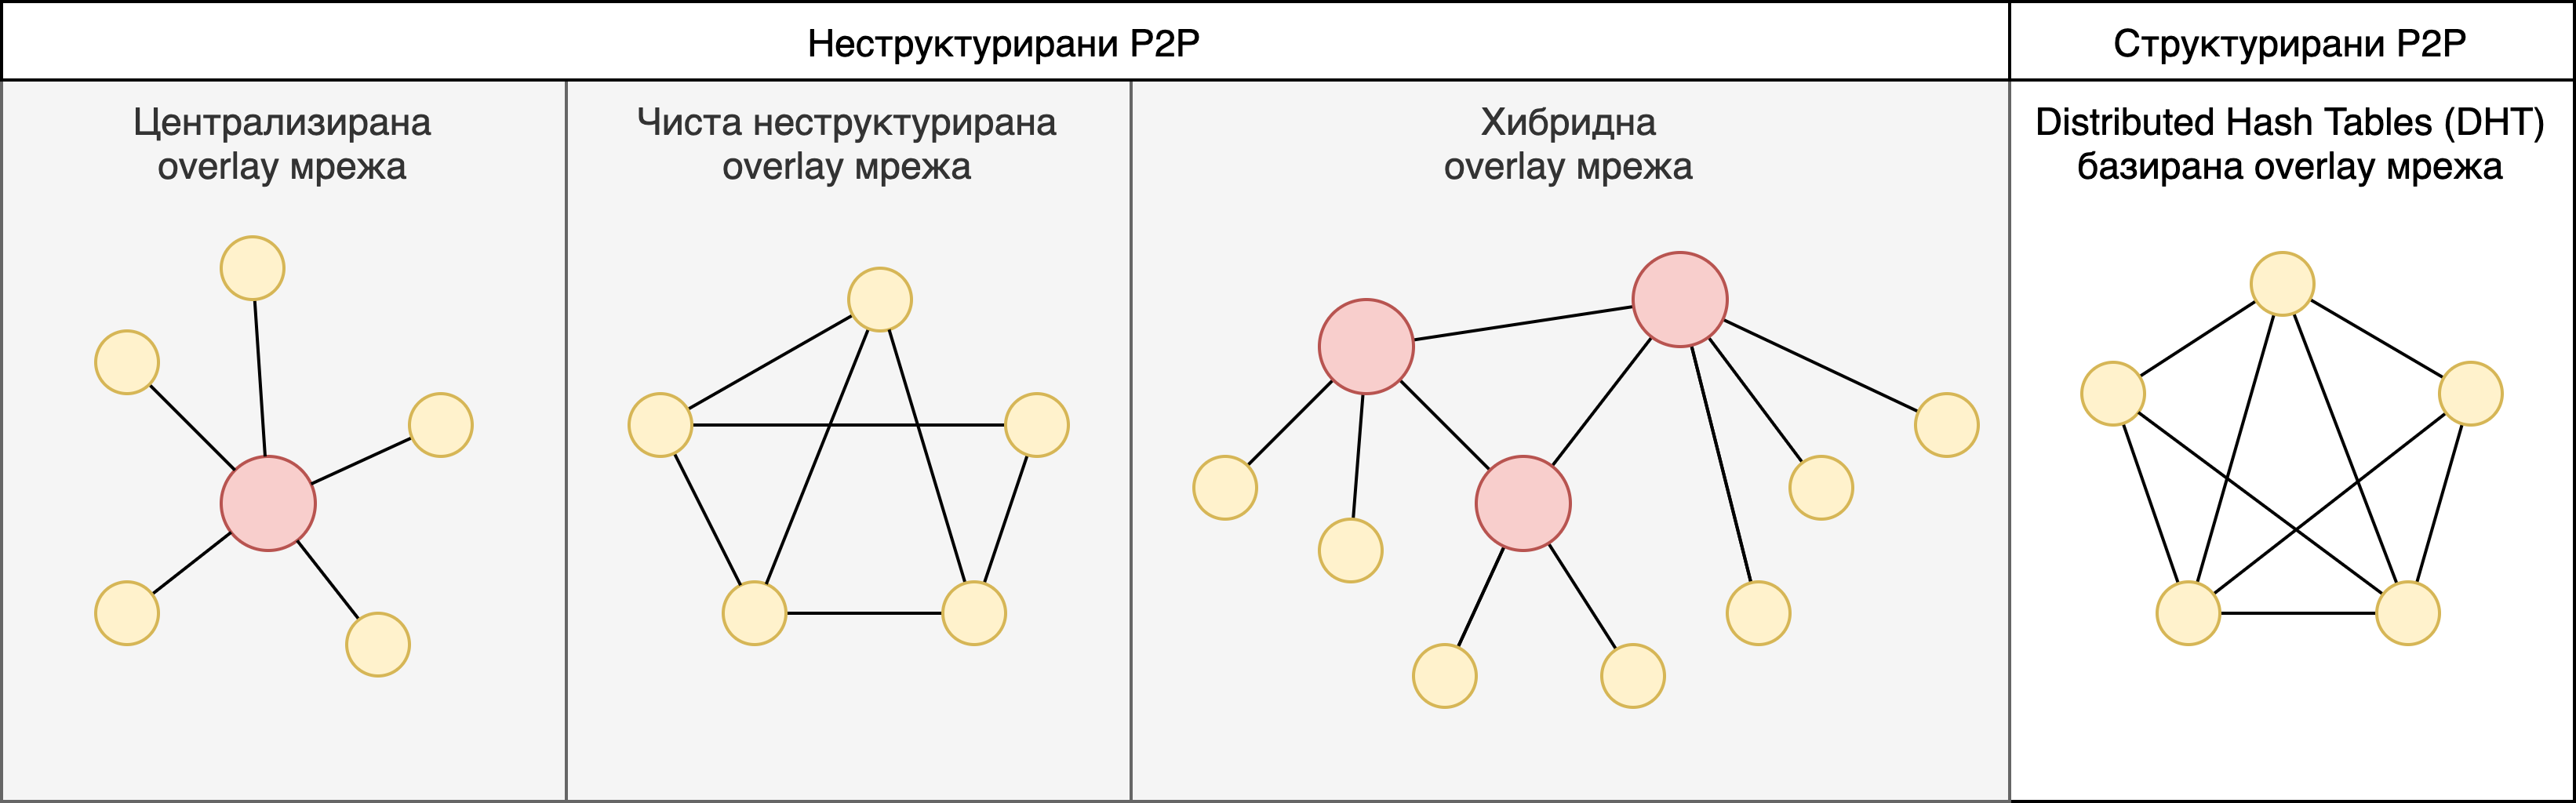
\includegraphics[width=500px]{p2p_overlay_topologies.png} \end{center}

\subsection{Сървъри за приложения и web-сървъри}

\textbf{\textit{Сървърът за приложения}} представлява съвкупност от компоненти, които могат да бъдат достъпни чрез платформено независими интерфейси за програмиране (\textbf{Application Programming Interface (API)}).
\textbf{\textit{Web-сървърите}} са вид сървъри за приложения, утилизиращи протокола \textbf{HTTP(S)}, където съдържанието, което се доставя, е основно \textbf{HTML} текст, но може да съдържа файлове дефинирани съгласно \textbf{MIME}.

\subsection{Метасистеми и грид}

Разпределените системи, могат да бъдат разделени в две категории в зависимост от свързаността и подобието на възлите си:
\begin{itemize}
    \item \textbf{клъстери} - локална мрежа от няколко хомогенни възела.
    \item \textbf{грид} - мрежа от хомогенни или хетерогенни възли, работещи заедно върху сложна задача, но разделени от големи дистаниции.
\end{itemize}

\subsection{Сервизно-ориентирани архитектури}

\textbf{\textit{Сервизно-ориентираната архитектура (Service-oriented architecture (SOA))}} е архитектурен стил където компонентите се третират като черни кутии наречени \textbf{услуги}.
\textbf{Услуга} дефинираме като самостоятелна единица, покриваща функционален домейн, която може да бъде достъпена отдалечено.
Тя може да бъде използвана посредством унифициран програмен интерфейс наречен \textbf{Application Programming Interface (API)}.

\subsection{Моделно-ориентирани архитектури}

\textbf{\textit{Моделно-ориентираната архитектура (Model-driven architecture (MDA))}} е софтуерна архитектура за автоматизирано проектиране на приложения.
Базира се на принципите на \textbf{model-driven engineering}, т.е. изграждането на абстрактни модели, които описват системата.
Целите на тази архитектура са разделянето на дизайна от конкретната имплементация.

\subsection{Аспектно-ориентирани архитектури}

\textbf{\textit{Аспектно-ориентираната архитектура}} е софтуерна архитектура, която се базира на принципите на \textbf{аспектно-ориентираното програмиране}.
При декомпозиция на модулите се появяват някои изисквания, които не могат да бъдат адекватно обособени в отделни компоненти.
Такива изисквания наричаме аспекти, като те представляват функционалности споделени между няколко компонента.
Такива са например изисквания свързани с audit logging.
Обичайно се имплементират чрез инжектиране на код в някои функции.

\subsection{Софтуерни агенти}

Софтуерните агенти са автономни софтуерни единици, които могат да изпълняват задания по заръка на своя хост.
Те се дефинират от гледна точка на своето поведение.
Присъщи техни характеристики са:
\begin{itemize}
    \item \textit{персистентност} - изпълняват се постоянно като демони и сами преценяват кога да предприемат действия.
    \item \textit{автономност} - могат да извършват задачи самостоятелно.
    \item \textit{социалност} - могат да взаимодействат с други компоненти чрез комуникация.
    \item \textit{реактивност} - агентите възприемат контекста, в който оперират и реагират спрямо него.
\end{itemize}

\end{document}
